\chapter{Deuteronomy 14}

\begin{figure}
  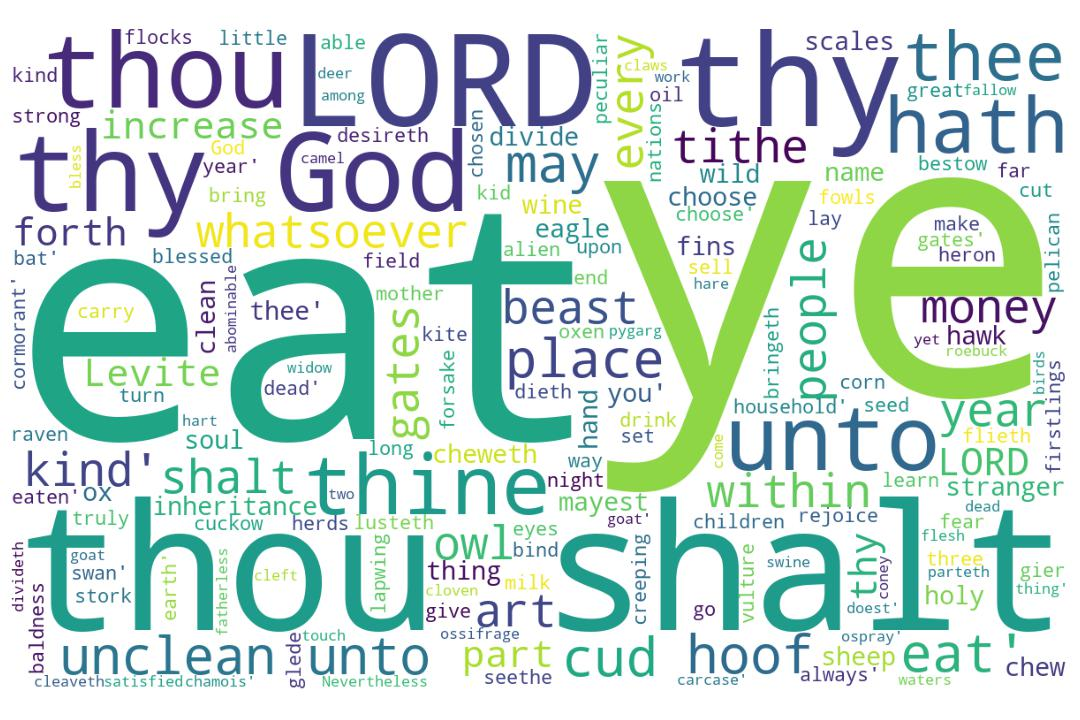
\includegraphics[width=\linewidth]{05OT-Deuteronomy/Deuteronomy14-WordCloud.jpg}
  \caption{Deuteronomy 14 Word Cloud}
  \label{fig:Deuteronomy 14 word Cloud}
\end{figure}

\marginpar{\scriptsize \centering \fcolorbox{bone}{lime}{\textbf{DETAILS}}\\ (Deuteronomy 14:1-29) \begin{compactenum}[I.][8]
    \item  \textbf{Prohibited Foods}  \index[scripture]{Deuteronomy!Deu 14:01--21}(Deu 14:1--21)
    \item  A \textbf{Peculiar People}  \index[scripture]{Deuteronomy!Deu 14:02}(Deu 14:02)
    \item  \textbf{Personal Hygiene}  \index[scripture]{Deuteronomy!Deu 14:08}(Deu 14:08)
    \item  \textbf{Preditory Birds}  \index[scripture]{Deuteronomy!Deu 14:12--19}(Deu 14:12--19)
    \item  \textbf{Prescribed Giving Foods}  \index[scripture]{Deuteronomy!Deu 14:28}(Deu 14:28)
    \item  \textbf{Protective Measures}  %\index[scripture]{Deuteronomy!Deu 14:28}(Deu 14:28)
\end{compactenum}}



\footnote{\textcolor[cmyk]{0.99998,1,0,0}{\hyperlink{TOC}{Return to end of Table of Contents.}}}\footnote{\href{https://audiobible.com/bible/deuteronomy_14.html}{\textcolor[cmyk]{0.99998,1,0,0}{Deuteronomy 14 Audio}}}\textcolor[cmyk]{0.99998,1,0,0}{Ye \emph{are} the children of the LORD your God: ye shall not cut yourselves, nor make any baldness between your eyes for the dead.}
[2] \textcolor[cmyk]{0.99998,1,0,0}{For thou \emph{art} an holy people unto the LORD thy God, and the LORD hath chosen thee to be a \fcolorbox{bone}{lime}{peculiar people} unto himself, above all the nations that \emph{are} upon the earth.}\\
\\
\P \textcolor[cmyk]{0.99998,1,0,0}{Thou \underline{shalt} not eat any \fcolorbox{bone}{lime}{abominable thing}.}
[4] \textcolor[cmyk]{0.99998,1,0,0}{These \emph{are} the beasts which ye shall eat: the ox, the sheep, and the goat,}
[5] \textcolor[cmyk]{0.99998,1,0,0}{The hart, and the roebuck, and the fallow deer, and the wild goat, and the pygarg, and the wild ox, and the chamois.}
[6] \textcolor[cmyk]{0.99998,1,0,0}{And every beast that parteth the hoof, and cleaveth the cleft into two claws, \emph{and} cheweth the cud among the beasts, that ye shall eat.}
[7] \textcolor[cmyk]{0.99998,1,0,0}{Nevertheless these ye shall not eat of them that chew the cud, or of them that divide the cloven hoof; \emph{as} the camel, and the hare, and the coney: for they chew the cud, but divide not the hoof; \emph{therefore} they \emph{are} unclean unto you.}
[8] \textcolor[cmyk]{0.99998,1,0,0}{And the swine, because it divideth the hoof, yet cheweth not the cud, it \emph{is} unclean unto you: ye shall not eat of their flesh, \fcolorbox{bone}{lime}{nor touch} their dead carcase.}\\
\\
\P \textcolor[cmyk]{0.99998,1,0,0}{These ye shall eat of all that \emph{are} in the waters: all that have fins and scales shall ye eat:}
[10] \textcolor[cmyk]{0.99998,1,0,0}{And whatsoever hath not fins and scales ye may not eat; it \emph{is} unclean unto you.}\\
\\
\P \textcolor[cmyk]{0.99998,1,0,0}{\emph{Of} all clean birds ye shall eat.}
[12] \textcolor[cmyk]{0.99998,1,0,0}{But these \emph{are} \emph{they} of which ye shall not eat: the \fcolorbox{bone}{lime}{eagle}, and the \fcolorbox{bone}{lime}{ossifrage}, and the \fcolorbox{bone}{lime}{ospray},}
[13] \textcolor[cmyk]{0.99998,1,0,0}{And the glede, and the kite, and the vulture after his kind,}
[14] \textcolor[cmyk]{0.99998,1,0,0}{And every raven after his kind,}
[15] \textcolor[cmyk]{0.99998,1,0,0}{And the owl, and the night hawk, and the cuckow, and the hawk after his kind,}
[16] \textcolor[cmyk]{0.99998,1,0,0}{The little owl, and the great owl, and the swan,}
[17] \textcolor[cmyk]{0.99998,1,0,0}{And the pelican, and the gier eagle, and the cormorant,}
[18] \textcolor[cmyk]{0.99998,1,0,0}{And the stork, and the heron after her kind, and the lapwing, and the bat.}
[19] \textcolor[cmyk]{0.99998,1,0,0}{And every creeping thing that flieth \emph{is} unclean unto you: they shall not be eaten.}
[20] \textcolor[cmyk]{0.99998,1,0,0}{\emph{But} \emph{of} all clean fowls ye may eat.}\\
\\
\P \textcolor[cmyk]{0.99998,1,0,0}{Ye shall not eat \emph{of} any thing that dieth of itself: thou \underline{shalt} give it unto the stranger that \emph{is} in thy gates, that he may eat it; or thou mayest sell it unto an alien: for thou \emph{art} an holy people unto the LORD thy God. Thou \underline{shalt} not seethe a kid in his mother's milk.}
[22] \textcolor[cmyk]{0.99998,1,0,0}{Thou \underline{shalt} truly tithe all the increase of thy seed, that the field bringeth forth year by year.}
[23] \textcolor[cmyk]{0.99998,1,0,0}{And thou \underline{shalt} eat before the LORD thy God, in the place which he shall choose to place his name there, the tithe of thy corn, of thy wine, and of thine oil, and the firstlings of thy herds and of thy flocks; that thou mayest learn to fear the LORD thy God always.}
[24] \textcolor[cmyk]{0.99998,1,0,0}{And if the way be too long for thee, so that thou art not able to carry it; \emph{or} if the place be too far from thee, which the LORD thy God shall choose to set his name there, when the LORD thy God hath blessed thee:}
[25] \textcolor[cmyk]{0.99998,1,0,0}{Then \underline{shalt} thou turn \emph{it} into money, and bind up the money in thine hand, and \underline{shalt} go unto the place which the LORD thy God shall choose:}
[26] \textcolor[cmyk]{0.99998,1,0,0}{And thou \underline{shalt} bestow that money for whatsoever thy soul lusteth after, for oxen, or for sheep, or for wine, or for strong drink, or for whatsoever thy soul desireth: and thou \underline{shalt} eat there before the LORD thy God, and thou \underline{shalt} rejoice, thou, and thine household,}
[27] \textcolor[cmyk]{0.99998,1,0,0}{And the Levite that \emph{is} within thy gates; thou \underline{shalt} not forsake him; for he hath no part nor inheritance with thee.}\\
\\
\P \textcolor[cmyk]{0.99998,1,0,0}{At the end of three years thou \underline{shalt} \fcolorbox{bone}{lime}{bring forth} all the tithe of thine increase the same year, and \underline{shalt} lay \emph{it} up within thy gates:}
[29] \textcolor[cmyk]{0.99998,1,0,0}{And the Levite, (because he hath no part nor inheritance with thee,) and the stranger, and the fatherless, and the widow, which \emph{are} within thy gates, shall come, and shall eat and be satisfied; that the LORD thy God may bless thee in all the work of thine hand which thou doest.}